\section{Sliding window protocol}
In \autoref{subsec:data-format} it was decided that the format of timestamps would be an integer from 0-255, where 0 to 20 would be considered as newer timestamps than 235 to 255.
However, if all the timestamps from 0 to 20 were lost, there would not be any updates until it has iterated through all other timestamps and back to 0.
To find a better solution to this problem the sliding window protocol was researched.
\\\\
Sliding window protocols are often used where reliable data is required, which means making sure that all data points are received.
This protocol uses window sized buffer space, where the window is a fixed number and the sender will send this number of the packets to the receiver \cite{design-and-validation-of-computer-protocols}.
Whenever the sender has sent the same number of packets as the size of the window, it waits for acknowledgements that the receiver has received the packets before sending additional packets.
Each packet gets a sequence number and the acknowledgement that is sent back also contains the sequence number.
By doing this the receiver can keep track of the packets, remove duplicates, identify missing packets and know which order is the correct one.
\\\\
On \autoref{fig:sliding-window} there is an illustration of a sliding window, where the window size is three.
In the first frame three packets are sent to the receiver, in the second frame the receiver has acknowledged all three packets, but the first acknowledgement fails.
The sliding window for the receiver has moved its window, but as the sender only has recieved acknowledgements from the second and third packet, it is unable to move its window and instead sends the first packet again in the third frame.
In the fourth frame the first packet has been acknowledged, and therefore the sliding window is moved for the sender and the sender is now able to send new packets.
\begin{figure}[H]
    \centering
    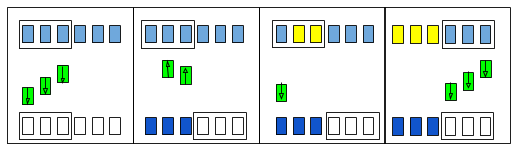
\includegraphics[width=\linewidth]{sliding-window-illustration.png}
    \caption{Sliding window protocol illustration where the top is the sender and the bottom is the receiver.}
    \label{fig:sliding-window}
\end{figure}
\noindent
For our project reliable data in the format of goal zones and goal score is important, however the reliability of player positions are not important.
The reasoning for this is explained in \autoref{subsubsec:choosing-between-udp-or-tcp}.
With Sliding Window protocol a player position would be retransmitted if it previously failed, and this position would now be outdated because the player might have moved since then.
TCP also already uses sliding window for flow control so for goal zones and goal score it is not necessary to implement, as these use TCP \cite{ibm:sliding-window}.
